\documentclass[a4paper,12pt]{llncs}
\usepackage[usenames,dvipsnames]{color}
\usepackage{graphicx}
\usepackage{subfigure}
\usepackage{listings}
\usepackage{color}
\usepackage{url}

\title{ISRuPIN-Win: Porting Instruction-Set Randomization Using Intel PIN Tool To Windows}
\author{Muhammad Ali Akbar (\texttt{UNI: maa2206})\\Supervision: Georgios Portokalidis and Angelos D. Keromytis\\
\email{maa2206@columbia.edu}
\institute{Computer Science Department,\\ Fu Foundation School of Engineering \& Applied Sciences,\\ Columbia University, NY}}

\begin{document}

\maketitle
\pagebreak

\section{Introduction}
\label{sec:intro}
Instruction Set Randomization (ISR) is a technique used to counter code injection attacks. It works by randomizing the instructions understood by the system, making it difficult for an attacker to guess the right set of instructions to carry out an attack. Invalid instructions are readily trapped by the operating system, resulting in process termination.

Randomization using a 16-bit XOR key changes the instruction set as follows. A typical \texttt{xor eax, eax} instruction maps to the opcode \texttt{33 C0} on an x86 system. However, if we randomize it with the key \texttt{DE AD}, an attacker would need to inject \texttt {ED 6D}; changing the key to \texttt{CA FE} will change the correct opcode to \texttt{F9 3E}. If the key is regenerated randomly and the executable code is randomized periodically with the new key, it makes the task of a malware writer extremely difficult as (s)he has no way of guessing the right code for the instruction and change it with each key change without knowing the actual key.

In \cite{portokalidis2010fast}, a fast and reliable implementation of ISR is presented. With the help of Intel's dynamic instrumentation tool known as PIN \cite{luk2005pin}, the proposed system randomizes an executable using randomly generated 16-bit XOR keys. It controls the execution of the executable and de-scrambles the instructions at runtime. Empirical experiments show a low overhead for the system as compared to the native execution. However, the system is limited to ELF executables and libraries for Linux.

Given the enormous market share that Microsoft Windows holds which is a huge incentive for commodity software development on Windows \cite{economides2006linux}, it is imperative that this system needs to be ported to Windows as well. This work is a step towards this direction. We have ported the ISR system presented in \cite{portokalidis2010fast} to native Windows environment. We use native Windows API to perform the same function as the Linux environment. Our system supports PE executable format, and has been tested on Windows 7.

\pagebreak

\section{Configuring \& Using ISRuPIN-Win}
\label{sec:design}
This section describes the configuration and working of the components of the system. The system consists of five modules, which are described below:

\subsection{objcopy: Randomizing the PE file}
This is the modified version of objcopy. The original source file,
the modified source file, the diff patch, and the binary executable are included.

\textbf{Description:}
Objcopy takes a binary executable and creates a copy of it in the specified binary format. It supports a wide variety of formats including ELF and PE binaries. With the current patch, the objcopy can randomize the TEXT section of both PE and ELF format executables using the specified 16-bit XOR key.

\textbf{Pre-requisites:}

1. From binary: To run the included binary executable, you just need to
install cygwin, and run this executable from cygwin's bash terminal.

2. From source: To recompile objcopy, you will need to get cygwin, install gcc and make.
Then, get the binutils-2.21.1 source code, replace/patch the objcopy.c file
and compile it.

\textbf{Usage:}

{\small \texttt{./objcopy --encrypt-xor-key [KEY] [input-file] [output-file]}}

For example,

{\small \texttt{./objcopy --encrypt-xor-key 0xDEAD input.exe encrypted-output.exe}}

\subsection{ida: Generating patch (Separating interleaved DATA from CODE section)}
This is a python script that uses IDA to generate patch file specifying
the jumptables (DATA in the .text section).

\textbf{Description:}
ELF executables have a clean separation between CODE and DATA. Unfortunately, the same is not true for PE executables. For example, the jump tables (DATA) is embedded right at the end of the function's code. Randomizing the whole TEXT section randomizes these jump addresses as well. This module is used to separate the DATA from CODE in the text section and create a patch file specifying the DATA blocks boundaries.

\textbf{Pre-requisites:}
IDA Pro (Tested on v6).

\textbf{Usage:}

Open the original (non-encrypted) PE file with IDA. Wait till initial
auto-analysis finishes. Run the python script from IDA (File $\rightarrow$ script file).
In the output window, click on each result and verify that there is no
false positive. If there is a false positive, you can fix it by telling
IDA to convert it to code and then function. Run the script again, a
patch file would have been generated (isr.func.patch).

\subsection{apply\_isr\_patch: Patching Randomized PE File}
This is the source code of the apply\_isr\_patch module.

\textbf{Description:}
It reads the patch file,
parses the input PE file, converts the virtual addresses in patch file
to raw offset within PE file, and then patches the corresponding bytes
in the output file.

\textbf{Pre-requisites:}

1. From binary: The compiled executable can be found here:

{\small \texttt{apply\_isr\_patch{\textbackslash}Debug{\textbackslash}apply\_isr\_patch.exe}}

2. From source: The visual studio project with the source code is attached. It has been created
and compiled using Visual Studio 2008.

\textbf{Usage:}

{\small \texttt{apply\_isr\_patch.exe xor\_encryption\_key input\_executable output\_executable patch\_file}}

\subsection{db: Updating ISRuPIN-Win Keys Database}
This is the sqlite database for storing the encryption keys. The sqlite3 client,
the database structure (sql) file, the database (db) file, and a script to
insert keys in to the database are attached.

\textbf{Pre-requisites:}
sqlite3.exe (included in the database folder).

\textbf{Usage:}
Change the \texttt{varenckey} and \texttt{varencname} parameters to the required key and executable path
in the insert\_key\_to\_db.bat file, and run it to insert the key in the image.

You can browse the database using the sqlite3 client by:

{\small \texttt{sqlite3.exe image\_keys.db}}

\subsection{isrupin-win: Run the program using pintool}
This is the source code of the isrupin (ISR pin tool for windows).

\textbf{Description:}
This is the main PIN tool. It loads binary executable and the dlls. It reads the corresponding keys from the
database. It sets up the instrumentation of the binary executable, and decodes the randomized binary instructions
on the fly as they are fetched. It uses a memory protector to separate the tool and executable's memory.

\textbf{Pre-requisites:}

1. From binary: The compiled pintool can be found here:

{\small \texttt{isrupin{\textbackslash}Debug{\textbackslash}isrupin.dll}}

2. From source: The visual studio project with the source code is attached. It has been created
and compiled using Visual Studio 2008.

\textbf{Visual Studio Configuration:}
The project has been configured with relative library addresses.
Get the pin-2.10-43611-msvc9-ia32\_intel64-windows PIN package,
and put the project folder (isrupin) at this location:

{\small \texttt{PIN\_FOLDER{\textbackslash}source{\textbackslash}tools{\textbackslash}MyWorkspace}}

Where PIN\_FOLDER is the folder where you extracted the PIN package.


\textbf{Usage:}

{\tiny \texttt{[FULL\_PATH\_TO\_PIN\_FOLDER]{\textbackslash}pin.bat -follow\_execv -t [FULL\_PATH\_TO\_PIN\_FOLDER]{\textbackslash}source{\textbackslash}tools{\textbackslash}MyWorkspace{\textbackslash}isrupin{\textbackslash}Debug{\textbackslash}isrupin.dll -unique\_logfile -keydb [FULL\_PATH\_TO\_DATABASE\_FOLDER]{\textbackslash}image\_keys.db -- [FULL\_PATH\_TO\_EXECUTABLE]}}

For example:

{\tiny \texttt{C:{\textbackslash}pin-2.10-43611-msvc9-ia32\_intel64-windows{\textbackslash}pin.bat -follow\_execv -t C:{\textbackslash}pin-2.10-43611-msvc9-ia32\_intel64-windows{\textbackslash}source{\textbackslash}tools {\textbackslash}MyWorkspace{\textbackslash}isrupin{\textbackslash}Debug{\textbackslash}isrupin.dll -unique\_logfile -keydb C:{\textbackslash}database{\textbackslash}image\_keys.db -- C:{\textbackslash}wamp32{\textbackslash}bin{\textbackslash}apache{\textbackslash}Apache2.2.21{\textbackslash}bin{\textbackslash}httpd.exe}}


\textbf{Formats supported:} PE executables (32 bit)

\textbf{Operating System:} Tested on Windows 7

\textbf{PIN version:} pin-2.10-43611-msvc9-ia32\_intel64-windows

\pagebreak

\section{Workflow}
\label{sec:workflow}
A workflow diagram that represents the steps required to randomize and run a PE using ISRuPIN-Win is given in Figure \ref{fig:workflow}.
\begin{figure}[!ht]
\centering
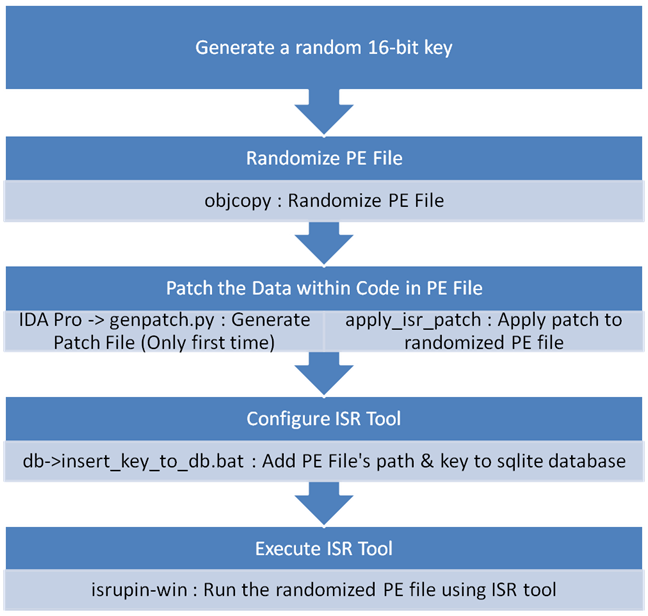
\includegraphics[scale=0.57]{workflow.png}\
\caption{Workflow Diagram}
\label{fig:workflow}
\end{figure}

The patch file generation (using IDA pro) needs to be done only once. This step can be skipped when re-encrypting the same binary with a different key. The patch file needs to be generated only if the binary changes. However, the randomized binary should be patched (using apply\_isr\_patch) every time the key is changed.

\pagebreak

\section{Challenges in Porting to Windows}
\label{sec:challenges}
Some of the important challenges we faced in porting ISRuPIN to windows are described below.

\subsection{Switching to Windows API}
For fast execution, it is imperative that ISRuPIN is run natively on Windows (without any emulation layer). For some cases, replacing Linux system calls with Windows API was straightforward. In other cases, we resorted to combining different APIs to perform the operations needed.

\subsection{No fixed System call numbers}
We want to track the memory usage of the executable in an attempt to separate its memory from the PIN tool's memory. Tracking specific system calls on Linux is easy, because the system call numbers are set in stone. Windows, on the other hand, treats system call numbers as another way to provide ASLR. System call numbers are changed in every minor Windows version. This is supposed to make it difficult for malware writers to make system calls using the system call table. This limits the tracking of memory management system calls. We had to resort to replacing the related API calls with wrapper functions using PIN API, and thus adding a level of indirection to be able to detect the required system calls. Note that this has to be done for each system call we want to monitor. We replaced this approach with a reactive one. Instead of monitoring memory management related system calls, we wait till we get a page fault, and then use Windows API to traverse the structure for allocated memory regions. This approach seems to work fast and efficient, as the traversal is done only on a hit, and the result is noted in an index of allowed memory regions for future use.

\subsection{`Not So Clean' Separation of Code and Data}
ELF executables have a clean separation between CODE and DATA. Unfortunately, the same is not true for PE executables. For example, the jump tables (DATA) is embedded right at the end of the function's code. Randomizing the whole TEXT section randomizes these jump addresses as well. This module is used to separate the DATA from CODE in the text section and create a patch file specifying the DATA blocks boundaries. We use Interactive Disassembler (IDA Pro) to disassemble the PE file and run a python script to identify the DATA blocks within TEXT section. Then, we parse the PE file using a custom C++ program, calculate offset in file corresponding to the virtual addresses, and patch those locations.

\subsection{No equivalent of procfs}
Windows doesn't have an equivalent of the virtual filesystem procfs that exports many kernel structures to the userspace. However, it does provide some decent API to walk through memory regions, shared modules etc, which almost makes up for the memory related information that procfs provides.

\subsection{Difficult to replace known system dlls}
Randomizing new dlls is easy as they can be placed in the executable's directory and will be loaded from there. However, Windows maintains a list of known dlls, and uses its own copy for known dlls even if they are not already loaded in memory. This makes it very difficult to replace the standard dlls with randomized ones without making this change for the whole operating system.

\section{Testing}
\label{sec:testing}
We tested the ISRuPIN-Win tool on several self written small programs. Testing was also done with programs that called Windows API and openssl library for encryption (both static and dynamic linking). The Apache web server (WAMP 32 bit windows distribution) was randomized and successfully tested with ISRuPIN-Win.

Some of the tools that we found helpful in debugging and testing were:

1. Text Logging from tool using PIN

2. Interactive Disassember (IDA Pro)

3. Diff tools (using VI, Windiff, VisualDiff etc)

4. Process Explorer


\section{Conclusion}
\label{sec:conclusion}
In this work, we have presented a port of ISR using PIN to Windows, described the workflow, discussed the challenges faced, and tested the implementation on real world production software.


\bibliography{biblio}{}
\bibliographystyle{splncs}

\end{document}


